\documentclass[12pt, a4paper]{article}

\usepackage{textcomp}
\usepackage{parskip}

% ===== Language and Encoding =====
\usepackage[utf8]{inputenc}
\usepackage[T1]{fontenc}
\usepackage[english]{babel}      % switch to "catalan" or "spanish" if needed

% ===== Page Layout =====
\usepackage[a4paper, margin=2.5cm]{geometry}
\usepackage{setspace}
\onehalfspacing                  % or \doublespacing if your uni requires it

% ===== Math =====
\usepackage{amsmath}
\usepackage{amssymb}
\usepackage{amsthm}
\usepackage{mathtools}
\usepackage{siunitx}             % for units, e.g. \SI{9.8}{\meter\per\second\squared}
\usepackage{upgreek}

\usepackage{chngcntr}
\counterwithin{equation}{section}


% ===== Graphics and Figures =====
\usepackage{graphicx}
\usepackage{subcaption}          % for subfigures
\usepackage{caption}
\captionsetup{font=small, labelfont=bf}

% ===== Tables =====
\usepackage{booktabs}            % professional-looking table rules
\usepackage{array}
\usepackage{multirow}
\usepackage{longtable}           % for tables spanning multiple pages

% ===== References and Citations =====
\usepackage[backend=bibtex, style=numeric, sorting=none]{biblatex}
\addbibresource{TFG.bib}  % your .bib file

% ===== Cross-referencing =====
\usepackage{hyperref}
\hypersetup{
    colorlinks=true,
    linkcolor=blue,
    citecolor=blue,
    urlcolor=blue,
    pdftitle={Your Thesis Title},
    pdfauthor={Your Name}
}
\usepackage[capitalize]{cleveref} % smarter \ref, use after hyperref

% ===== Code listings (if you need to show code snippets) =====
\usepackage{listings}

% ===== Miscellaneous =====
\usepackage{xcolor}
\usepackage{enumitem}             % more control over lists
\usepackage{appendix}
\usepackage{xurl}

\title{SUPERCONDUCTING ALUMINUM CPW $\lambda/4$ RESONATORS ON DIAMOND, 4H-SiC AND 6H-SiC SUBSTRATES FOR DIELECTRIC LOSS CHARACTERIZATION}
\author{Gabriel Vitagliano}
\date{August 2026}

\begin{document}

\maketitle

\newpage

\tableofcontents

\newpage

\section{Introduction}

\textcolor{red}{Uno de los principales avances de la aplicación de la física cuántica es la computación cuántica; en particular, la computación cuántica basada en circuitos superconductores. Esta consiste en el uso de bits cuánticos (qubits); los cuales, a diferencia de un transistor convencional, permiten estados intermedios entre el 1 y el 0 mediante la superposición de estados. Uno de los principales problemas que presentan este tipo de circuitos es el tiempo de coherencia; el cual se define como el tiempo que tarda un sistema en superposición en colapsar en uno de los estados que lo componen. Dicho concepto depende directamente de la cantidad física conocida como factor de calidad ($Q_L$). El factor de calidad puede entenderse como la cantidad de energía almacenada en el circuito relacionada con la cantidad de energía que pierde el circuito en cada "período de funcionamiento" de este.} 

\textcolor{red}{Desde el descubrimiento de la computación cuántica mediante circuitos superconductores, gran parte de la investigación relacionada a este tema ha sido alrededor de la maximización del tiempo de coherencia mencionado previamente; y por lo tanto, la optimización del factor de calidad de los circuitos utilizados. A pesar de esta tendencia, en la línea de investigación de circuitos superconductores es aparente que existe un límite en el $Q_L$ independiente de la configuración del circuito utilizado y de la calidad de fabricación de este.}

\textcolor{red}{La causa de este límite aparente es aún objeto de estudio, aunque aún así haya hipótesis sobre posibles fuentes de pérdida de energía en estos circuitos. Una causa posible es la generación de cuasipartículas dentro del superconductor; otra causa considerada es la incidencia de radiaciones cósmicas en el superconductor; y, finalmente, la causa que se estudiará principalmente en este trabajo, la presencia de sistemas de dos niveles (TLS) en las interficies entre metal y sustrato, los cuales interfieren en el mecanismo de la superconductividad.}

\textcolor{red}{En el trabajo a continuación se explicará el procedimiento, los resultados y la discusión de estos, realizados para el estudio exhaustivo del diamante, 4H-SiC y 6H-SiC como sustratos para la fabricación de circuitos superconductores en base a aluminio granular (grAl).}

\textcolor{red}{Dicho estudio consistirá en el diseño de un circuito superconductor basado en resonadores de línea de transmisión planares de tipo $\lambda/4$ CPW acoplados de manera inductiva a una línea de alimentación, también consistente en una línea de transmisión planar. Dicho diseño será luego simulado con el programa de método de momentos Sonnet, con el fin de aproximar parámetros fundamentales como la impedancia, la permitividad efectiva, frecuencia de resonancia y el factor de calidad externo ($Q_e$). Una vez realizadas las simulaciones y optimizado el diseño para el experimento en cuestión el circuito será fabricado por el grupo de "Name" en "Nombre de la universidad o instituto de Munich" para ser medido y caracterizado. A través de dichas mediciones se planean conseguir experimentalmente los parámetros estudiados inicialmente en las simulaciones.}

\textcolor{red}{El diseño del circuito a ser estudiado fue realizado de la siguiente manera: en primer lugar la elección de unos parámetros iniciales con los cuales se hace un primer estudio de los parámetros de interés. Luego, ajustar los parámetros en función de los resultados de las simulaciones. Y, finalmente, realizar un estudio de la respuesta del circuito a señales de diferentes frecuencias en el rango de microondas y, a través de dicha respuesta calcular el factor de calidad externo ($Q_e$).}

\textcolor{red}{El objetivo del diseño de cada chip es conseguir que cada resonador tenga un $Q_e$ de un orden de magnitud diferente, y dentro del rango esperado, para que se pueda conseguir al menos una señal apropiada independientemente del orden de magnitud del $Q_i$ real del circuito fabricado.}

The objective of the following piece of research was to follow on the issue discussed by \cite{Charpentier2025}, about the importance of the threshold reached for $Q_i$ for 2-dimensional superconducting circuits designed for quantum computing; especially due to losses coming from TLS in substrate-metal interfaces. The approach that was decided on was the design of a resonator circuit targeting the maximization of $Q_i$ while keeping a representative system for the desired use, which is Al thin film superconducting circuits; and simultaneously avoiding factors outside what strictly concerns the substrate-metal interfaces.

Because of the lack of research concerning the cryogenic-microwave properties of diamond, 4H-SiC and 6H-SiC an estimation of the resulting $Q_i$ proved to be difficult. As a result, the circuit was designed in such a way that several different values of $Q_e$ are explored so that it's more probable that a signal in the critically coupled regime could be achieved. This way, the resulting circuit for each substrate consists of a set of 4 $\lambda/4$ CPW resonators inductively coupled to a CPW feedline which is in turn connected to two launchers, one on each end.

These designs were simulated using the method of moments software Sonnet, which was useful for the calculation of the $\epsilon_r$ and $Z_0$, as well as the $f_r$ and making an estimation of the $Q_e$ from each simulated $S_{21}$ response.

\newpage

\section{Theory background}

In this chapter key theoretical concepts needed to understand the general workflow as well as to understand the results provided later on will be introduced. A section dedicated to general concepts of superconductivity will serve to understand the materials being used. Following this, a section describing the behavior of quarter-wave coplanar waveguide resonators will introduce and give a detailed explanation of the concepts and expressions used to make predictions for the overall design and analysis of the systems to be studied.

\subsection{Superconductivity} \label{Superconductivity}

This section will be dedicated to the explanation of specific concepts related to superconductivity relevant to this thesis. First, explaining basic phenomenology; then, touching on the subject of BCS theory and Cooper pairs; and finally, arriving at the concept of type I and type II superconductors.

\subsubsection{Basic phenomenology}

This section will follow the analysis shown by \cite{Annett2003}.

When talking about superconductivity, the first thought that comes to mind is conduction with a resistance exactly equal to zero; or rather, conduction with an infinite value of conductivity. And, even though this is, in reality, the most desirable key characteristic of superconducting materials due to the lack of resistive energy losses, the truth is that a completely pure metal with no impurities would also show this characteristic, as its temperature approached absolute zero, without being catalogued as a superconductor. The key differences between the two are as follows.

\begin{figure}[h]
    \centering
    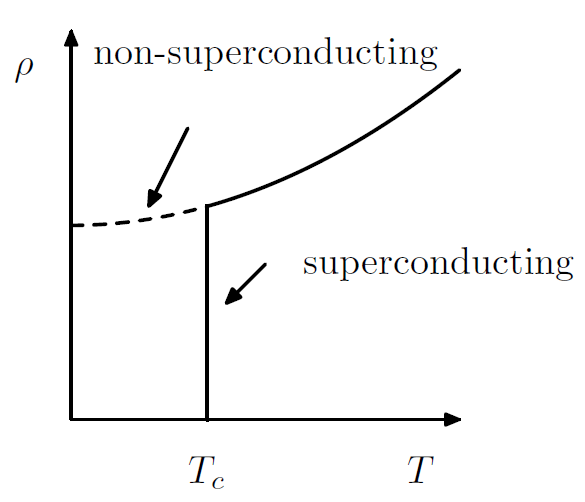
\includegraphics[width=0.6\textwidth]{figures/SuperConducting_Transition.png}
    \caption{Sudden drop in resistivity to zero at the critical temperature. Reproduced from \cite{Annett2003}}
    \label{fig:SupercondPhaseTrans}
\end{figure}

Firstly, a true superconductor experimentally shows a sudden drop in resistivity to exactly zero as shown in \cref{fig:SupercondPhaseTrans}, at a given temperature called the critical temperature of a superconductor ($T_c$). This sudden drop, is an indicator of a clear phase transition between what is called a normal conductor and a superconductor.

\begin{figure}[h]
    \centering
    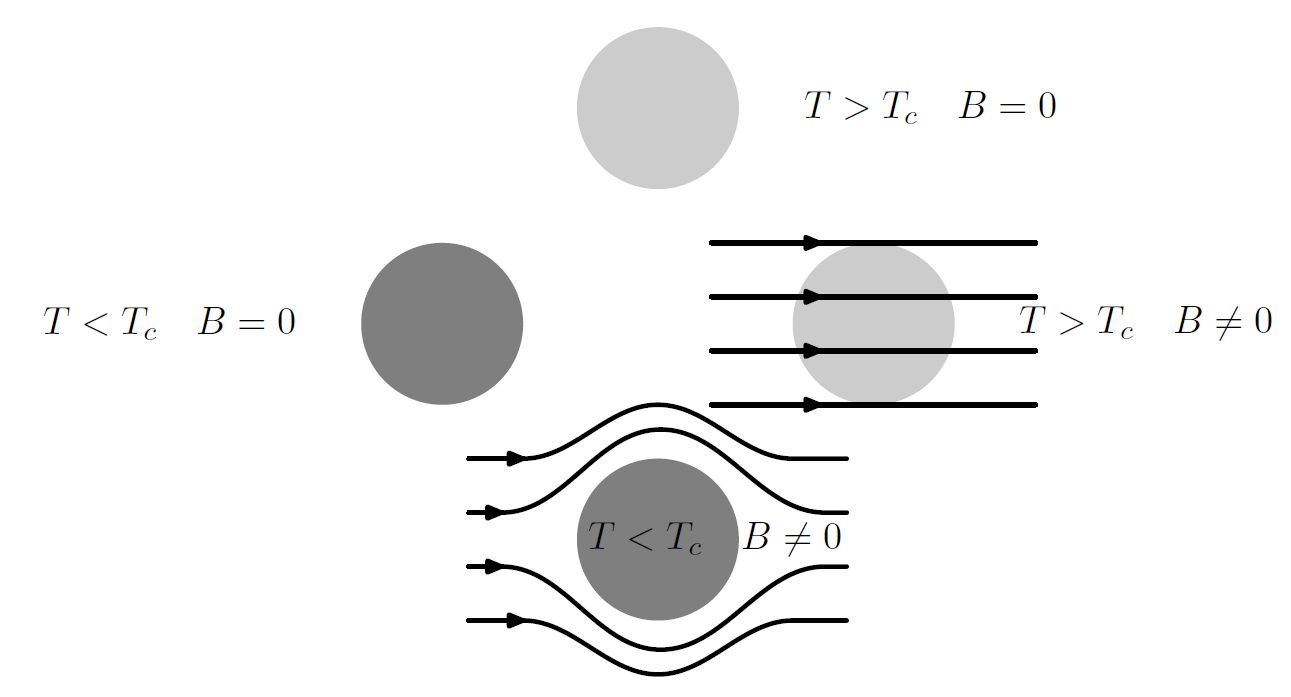
\includegraphics[width=0.6\textwidth]{figures/Meissner_Oschenffeld.png}
    \caption{Meissner Ochsenfeld effect representation. Reproduced from \cite{Annett2003}}
    \label{fig:MeissnerOchsenfeld}
\end{figure}

Additionally, in the case of a superconductor, once the critical temperature is achieved, the magnetic field inside the material also becomes exactly zero; this phenomenon is called the Meissner-Ochsenfeld effect. The Meissner-Ochsenfeld effect consists in a phenomenon where the superconducting material arrives at the same state of equilibrium with $B = 0$ inside it independently of its previous state, as shown in \cref{fig:MeissnerOchsenfeld}. This means that whether there was an existing external magnetic field traversing the material or not, does not matter to its final state. It is worth noting that if the material did have an external magnetic field $H$ going through its volume, in order to expel it, it will become magnetized the opposite way such as $M = -H$; this is why superconductors can also be considered perfect diamagnets ($\chi = -1$).

Considering that the measurement of resistivity employs the use of material that would add resistivity difficult to exclude from the results, the Meissner effect is the preferred experimental way of proving that a certain material does, in fact, present superconductivity; since the measurement of magnetization proves to be less invasive to the material.

\subsubsection{London penetration depth and superconductivity types}

Of interest to this thesis is the classification of superconductors into two types, Type-I and Type-II, based on their response to external magnetic fields \cite{Annett2003}. 

\begin{figure}[h]
    \centering
    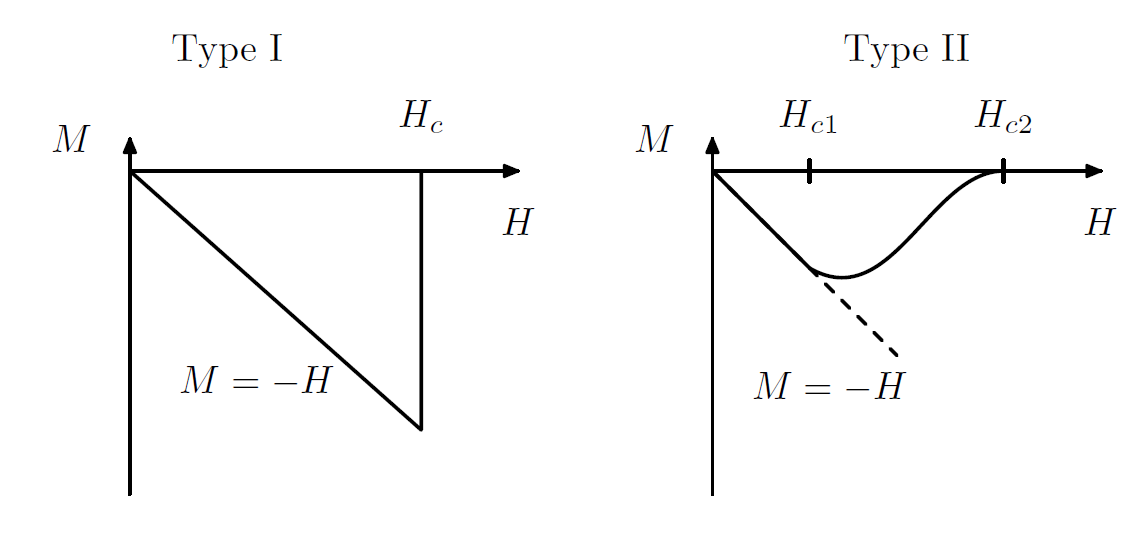
\includegraphics[width=0.6\textwidth]{figures/TypeI_TypeII.png}
    \caption{Reproduced from \cite{Annett2003}}
    \label{fig:SupcondTypes}
\end{figure}

In a Type-I superconductor, the same way there exists a critical temperature $T_c$ or a critical electrical current $I_c$ for which superconductivity is suddenly broken, there exists a critical magnetic field $H_c$ for which resistivity ceases to be exactly zero and the Meissner effect ceases to occur. This means that the material's magnetization becomes zero as it is represented in \cref{fig:SupcondTypes}, and therefore the lines of the external field $H$ suddenly penetrate the material normally.

\begin{figure}[h]
    \centering
    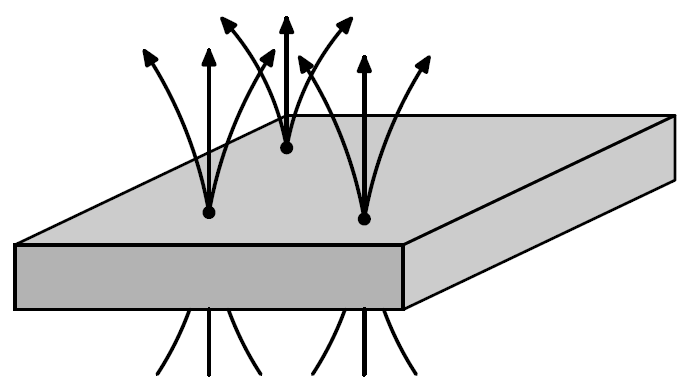
\includegraphics[width=0.6\textwidth]{figures/Vortices.png}
    \caption{Reproduced from \cite{Annett2003}}
    \label{fig:Vortices}
\end{figure}

On the other hand, on a Type-II superconductor this transition towards normal conductivity is much smoother. In this case, rather than taking one critical magnetic field $H_c$, two critical field values are studied, $H_{c1}$ that represents the value of $H$ for which $M$ stops strictly behaving as $M = - H$; and $H_{c2}$ that represents the value of $H$ for which $M$ exactly zero. As a consequence of this behavior, magnetic flux is able to partially penetrate the material in the interval between $H_{c1} \text{ and } H_{c2}$, in the form of discrete flux vortices as it is represented in \cref{fig:Vortices}.

Around these vortices the magnetic field decays radially over the characteristic length known as the London penetration depth $\lambda_L$. In the context of this thesis, it is notable how this quantity might behave in thin-film superconductors.

According to \cite{Lopez-Nunez2025}, when a thin-film's thickness is smaller than the mean free path $l$\footnote[1]{In the context of superconductors, the mean free path is defined as the characteristic length in between collisions between quasiparticle pair-constituent electrons and discontinuities such as phonons or impurities in the material \cite{Tinkham1996}.}, the mean free path behaves such as $l \approx t$ where $t$ is the thickness of the metallic film. This is consequential, as the value of the effective $\lambda$ in the dirty superconductor limit\footnote[2]{In general, evaporated Al thin films work in this regime, as the Al bulk coherence length is $\xi_0 = 1.6 \mu m$.} ($\xi_0\footnotemark[3]\gg l$)\footnotetext[3]{$\xi$ is defined as the coherence length; which corresponds to the length after a collision where the order parameter is recovered \cite{Tinkham1996}} depends on $l$ such as

\begin{equation}
    \label{LondonDepth}
    \lambda = a \lambda_L \sqrt{\frac{\xi_0}{l}}.
\end{equation}

Where $a$ depends on the surface scattering type ($a \approx 1.33 \text{ for diffusive scattering, and } a \approx 1.15 \text{ for specular reflection}$ \cite{Tinkham1996}). This way, the effective penetration depth $\lambda$ becomes bigger as the thickness of the thin-film is reduced. This way, \cite{Lopez-Nunez2025} discusses how the thickness of the thin-film can be related to a transition in the superconductivity type of aluminum. In particular, they discuss how as the thickness of the film becomes larger, in an interval of [54nm, 207nm], the apparition of flux vortices decreases up to a point where the material appears to become a Type-II superconductor. This phenomenon gets also attributed to other aspects of the geometry of the film; in this case, the geometry of the resonators, including the ratio between the thickness of the film and the width of the conductor of the CPW resonators used for measurements. 

\subsubsection{BCS theory and quasiparticles}

In order to better understand the mechanisms of superconductivity, an understanding of the microscopic physics behind the behavior of these materials is needed. The Bardeen, Cooper and Schrieffer (BCS) theory, through the use of quantum many-body theory, does a good job at explaining and predicting the experimentally known phenomena surrounding superconductivity \cite{Annett2003}.

This framework treats the interactions between electrons inside the superconductor through the combined effect of screened Coulomb repulsion and an attractive, phonon-mediated interaction, together acting on the wave-function of the entire body of electrons. The screened Coulomb repulsion between electrons takes the form

\begin{equation}
    \label{CooperPotential}
    V_{TF}(\mathbf{r}-\mathbf{r'}) = \frac{e^2}{4 \pi \epsilon_0 |\mathbf{r}-\mathbf{r'}|} e^{-|\mathbf{r}-\mathbf{r'}| / r_{TF}},
\end{equation}

which is overcome, within a narrow energy window near the Fermi surface, by the attractive interaction mediated by lattice phonons. The net result is a weak effective attraction between electrons near the Fermi level, responsible for the formation of Cooper pairs; which are bound states formed by two electrons sharing a common wave-function.

\begin{figure}
    \centering
    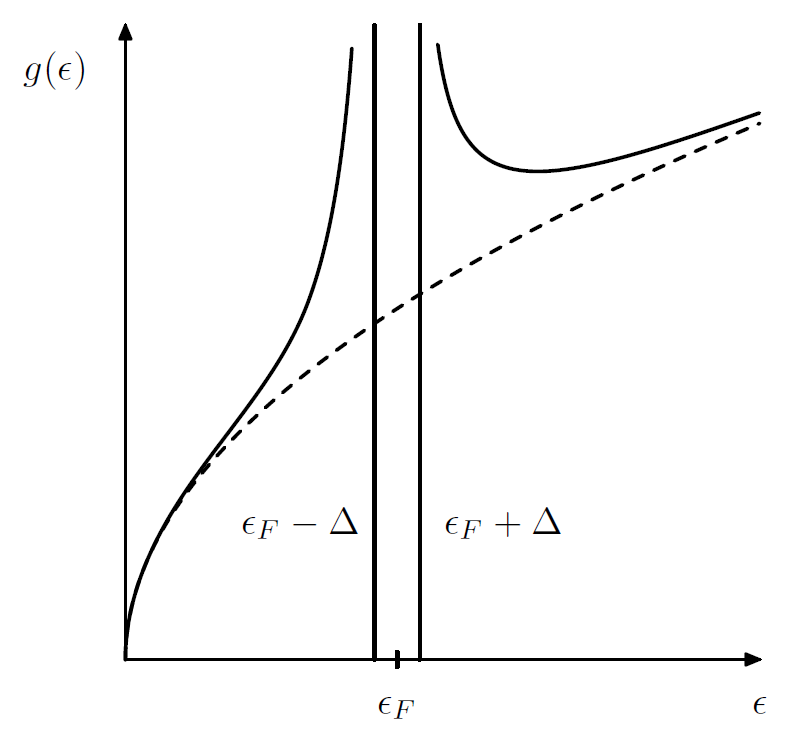
\includegraphics[width=0.6\textwidth]{figures/EnergyBandGap.png}
    \caption{Reproduced from \cite{Annett2003}}
    \label{fig:EnergyBandGap}
\end{figure}

This attractive interaction shows itself as a formation of an energy gap in the excitation spectrum, 

\begin{equation}
    \label{EnergyGap}
    2\Delta(0) = 3.52 k_B T_c,
\end{equation}

 which, as can be seen in \cref{fig:EnergyBandGap}, remains centered at the Fermi level. This result is especially notable, as it explains the robustness of the Cooper pair against dissipation.

Additionally, when one takes into account collisions with imperfections within the superconductor's volume or phonons, the results show a complex conductivity for the superconducting state \cite{Glover1957}

\begin{equation}
    \label{ComplexConductivity}
    \sigma = \sigma_1 + i \sigma_2.
\end{equation}

Where the real part represents the energy losses due to collisions with phonons with energy of the order of the energy gap \cref{EnergyGap}, as well as with imperfections in the material. These collisions can lead to Cooper pairs breaking, which produces two unpaired Bogoliubov quasiparticles. These quasiparticles behave closer to normal conductivity and therefore dissipate energy in an analogous manner to Ohmic losses.

\subsection{Quarter-wave coplanar waveguide resonators} \label{QWCPWR}

The following section will be dedicated to the theoretical explanation of the general behavior of quarter-wave coplanar waveguide resonators focusing on the mechanisms of resonance, resonance frequency, characteristic impedance, quality factor and energy loss mechanisms.

\subsubsection{General CPW physics} \label{GeneralCPW}

In order to understand the physics behind quarter-wave CPW resonators, one must first understand what a microwave resonator is.

Usually, when the wavelength of the electromagnetic signal used is much bigger than the size of the elements used to build a circuit (which is the case for domestic power transmission at around 50Hz, which translates to wavelengths of around 6000km), the lumped element model is used for the analysis of electric circuits. When working in this regime, it is possible to build resonators such as the RLC resonator. This system consists in a circuit containing a resistor, $R$, an inductor, $L$ and a capacitor $C$. Using these elements in different arrangements, it is possible to arrive to several different devices, the most emblematic of which, are the series and the parallel RLC resonators. 

As their name suggest, these circuits are characterized by the fact that the electric field generated by the capacitor and the magnetic field generated by the inductor both oscillate the same way a mechanical oscillator's kinetic and potential energy would oscillate. In this kind of oscillator, resonance is found at the frequency where the input impedance (which is defined as the complex ratio between voltage and alternating current) is purely real. This frequency shows to be such as

\begin{equation}
\label{lumpedresonance}
    \omega_0 = \frac{1}{\sqrt{LC}}.
\end{equation}

Similarly, when the size of the elements studied is comparable to the wavelength of the electromagnetic field (which is the case for the microwave spectrum, corresponding to wavelengths on the order of centimeters), the distributed-element model is used. This model describes a transmission line in terms of per-unit-length parameters resistance ($R'$), inductance ($L'$), conductance ($G'$), and capacitance ($C'$) assigned to infinitesimal segments of the line, analogous to the lumped-element model. Taking the continuum limit of these segments yields the telegrapher's equations, which govern voltage and current as functions of position along the line. This model takes into account how the voltage and subsequent current change along the surface of each element; revealing aspects of the circuit electrodynamics that are lost in lumped element circuitry.

In the case of the distributed element, the resonators most represented in the literature are resonant cavities, $\lambda/2$ CPW resonators and $\lambda/4$ CPW resonators. For the sake of this study, only the case of quarter-wave coplanar waveguide resonators will be explored.

For distributed-element structures with simple field symmetry, such as coaxial lines or parallel-plate capacitors, the per-unit-length capacitance, and hence $\epsilon_{eff}$ and $Z_0$, can be obtained directly from Gauss's law in closed form. Coplanar waveguides, however, lack this symmetry. This is because the electric field is distributed inhomogeneously between the substrate and the air above the slots, and no simple closed surface captures the geometry. Conformal mapping techniques, are therefore used to obtain closed-form expressions for $C'$ by mapping the CPW cross-section onto an equivalent geometry where the capacitance is tractable.

\begin{figure}
    \centering
    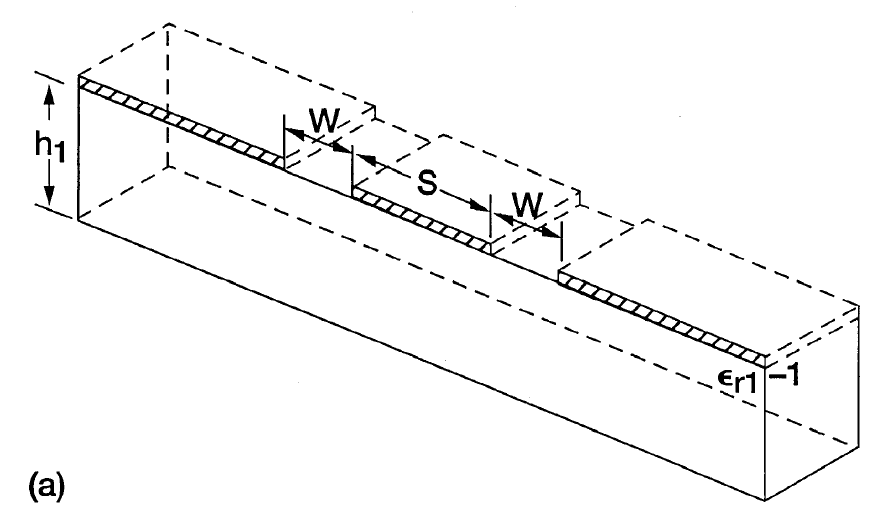
\includegraphics[width=0.4\textwidth]{figures/Conformal_a.png}
    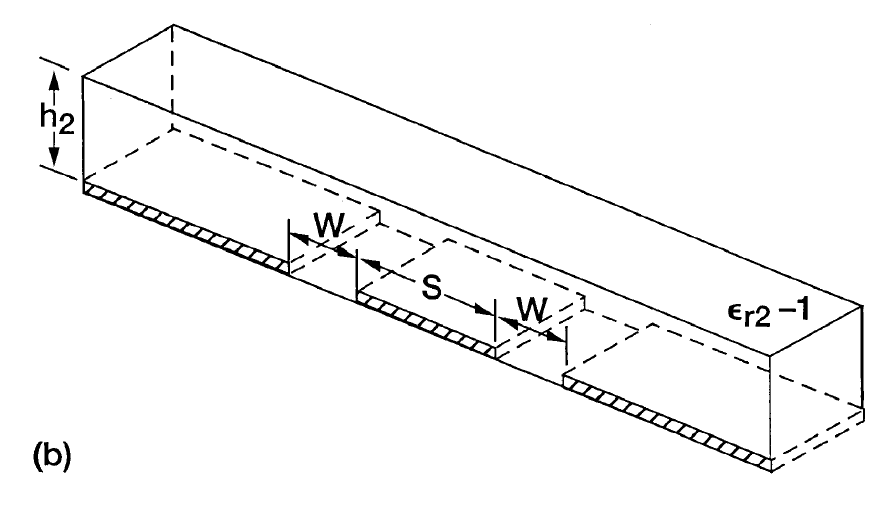
\includegraphics[width=0.4\textwidth]{figures/Conformal_b.png}
    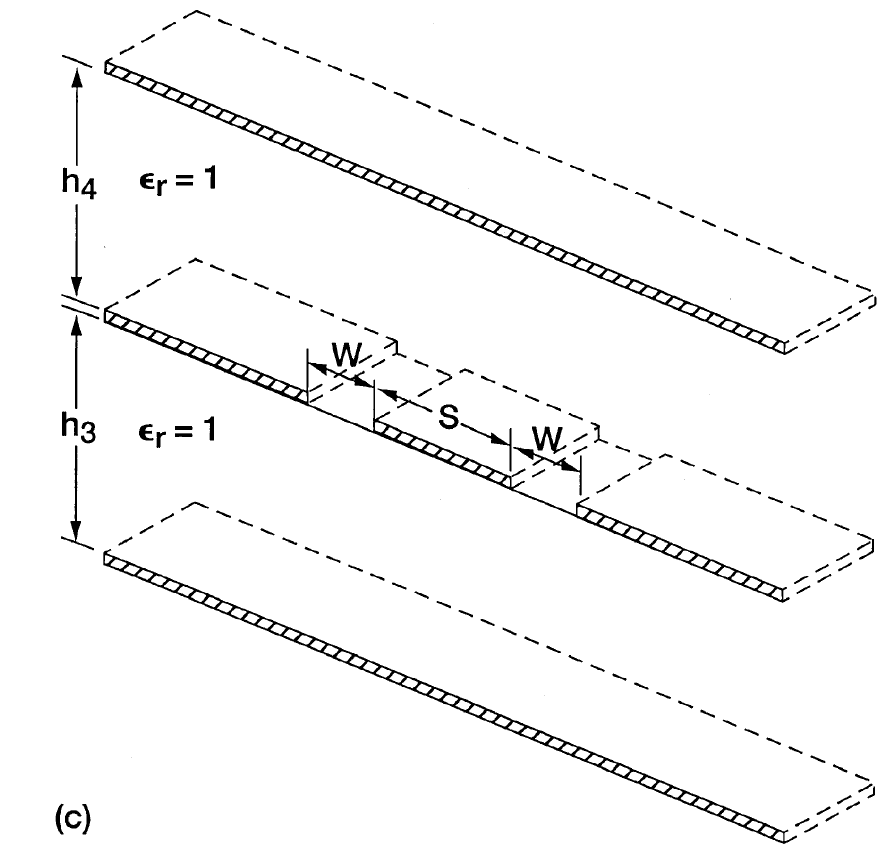
\includegraphics[width=0.4\textwidth]{figures/Conformal_c.png}
    \caption{Reproduced from \cite{RaineeN2001}}
    \label{fig:ConfMapping}
\end{figure}

In this particular case, conformal mapping proves useful as the equations to be described are the Laplace equations, which are notoriously invariant to conformal transformations. According to the results shown by \cite{Gevorgian1995} and \cite{RaineeN2001}, by using the Christoffel-Schwartz transformation in order to compute the total capacitance as the sum of the capacitances computed in the partial regions shown in \cref{fig:ConfMapping} such as:

\begin{equation}
    \label{capacitance}
    C_{CPW} = C_1 + C_2 + C_{air}.
\end{equation}

And using the following relationship \cite{Gevorgian1995}:

\begin{equation}
    \label{CapPerm}
    \epsilon_{eff} = \frac{C_{CPW}}{C_{air}}.
\end{equation}

One can arrive to the following results for the effective permittivity and the characteristic impedance when taking into account a coplanar waveguide with a grounded finite substrate \cite{Wadell1991}:

\begin{equation}
    \label{permittivity}
    \epsilon_{eff} = \frac{1 + \epsilon_{r} \frac{K(k'_0)}{K(k_0)} \frac{K(k_1)}{K(k'_1)}}{1 + \frac{K(k'_0)}{K(k_0)} \frac{K(k_1)}{K(k'_1)}}
\end{equation}

and

\begin{equation}
    \label{impedance}
    Z_0 = \frac{60\pi}{\sqrt{\epsilon_{eff}}}\frac{1}{\frac{K(k_0)}{K(k'_0)} + \frac{K(k_1)}{K(k'_1)}}
\end{equation}

Where $K(k_0)\text{, }K(k'_0)\text{, }K(k_1) \text{ and } K(k'_1)$ are complete elliptic integrals, whose modulus come given by:

\begin{subequations} \label{k_definition}
\begin{align}
    \label{ElipModulus}
    k_0 = a/b \\
    k'_0 = \sqrt{1 - k_0^2} \\
    k_1 = \frac{\tanh(\frac{\pi a}{4h})}{\tanh(\frac{\pi b}{4h}} \\
    k'_1 = \sqrt{1 - k_1^2}
\end{align}
\end{subequations}

As a result of this, the phase velocity of light through the circuit will as

\begin{equation}
    \label{vph}
    v_{ph} = \frac{c}{\sqrt{\epsilon_{eff}}}.
\end{equation}

Finally, if one considers a transmission line with an open end and a shorted end; which is equivalent to having boundary conditions of $Z(0) = 0 \text{ and } Z(l) \to \infty$; one arrives to the following condition \cite{Gao2008}

\begin{equation}
    \label{ResCond}
    l = (2n + 1) \frac{\lambda}{4}, \, n \in \mathbb{N}.
\end{equation}

Hence, the length of the resonator would be

\begin{equation}
    \label{length}
    l_{total} = \frac{v_{ph}}{4 \cdot f_r}.
\end{equation}

It is also worth noting the importance of properly taking into account the impedance in a resonator's design. According to \cite[Chapter~5]{Pozar2012}, the reflection coefficient near resonance of a quarter-wave CPW resonator is described as

\begin{equation}
    \label{ImpReflection}
    |\Gamma| \approx \frac{|Z_L - Z_0|}{2 \sqrt{Z_0 Z_L}} |\cos\theta|.
\end{equation}

Where $Z_0$ is the characteristic impedance of the transmission line, as seen in \cref{impedance}, and $Z_L$ is the loading impedance, which is defined as the impedance value terminating the transmission line; which in our case matches the impedance of the coaxial cable feeding the signal. Analyzing the expression, one can notice that the closer the characteristic impedance is to the load impedance, the lower the reflection coefficient will be, which is desirable when working with transmission readouts.

One way to study the resonance frequency and overall physics of a coplanar waveguide resonator circuit are scattering parameters, often represented through the scattering matrix such as \cite{Pozar2012}

\[
\begin{pmatrix}
    V^{-}_1\\
    V^{-}_2
\end{pmatrix}
=
\begin{pmatrix}
    S_{11} & S_{12}\\
    S_{21} & S_{22}
\end{pmatrix}
\begin{pmatrix}
    V^{+}_1\\
    V^{+}_2
\end{pmatrix}.
\]

In this notation, the subindices i and j stand for the input and the output port, and the superindices + and - refer to the direction from which a wave is arriving to a port (In this case + means the wave is going away from the port and - means it is coming into the port). The elements of the matrix can then be interpreted as reflection terms when $i = j$ and transmission terms when $i \neq j$. 

In the case of a quarter wave resonator, the main object of study is the behavior of the $S_{21}$ coefficient. This element of the scattering matrix represents the transmission of signal from the input port into the output port. In the case of the systems at hand, when resonance is achieved, a significant part of the energy going through the feedline gets transferred to the resonator, and thus leading to a dip in the $S_{21}$ coefficient. Exploring this behavior can prove rather useful to study characteristics of the circuit or the materials that conform it, such as capacitances, inductances, and energy losses.

\subsubsection{Quality factor and energy loss} \label{Qfactor}

Energy losses are mainly quantified using the concept of quality factor (Q). This concept is directly tied to the overall performance of a superconducting circuit. The loaded quality factor of a given circuit can be separated into several quality factors corresponding to the several loss mechanisms that can be found. This relationship can be expressed as \cite{Charpentier2025}

\begin{equation}
    \label{Q_L}
    Q^{-1}_{L} = Q^{-1}_{TLS} + Q^{-1}_{c} + Q^{-1}_{qp} + Q^{-1}_{vortex} + Q^{-1}_{rad} + \dots
\end{equation}

Even though there is a great quantity of energy loss channels, for the sake of this study only the ones shown will be explained; going into greater detail for $Q_{TLS} \text{, } Q_{vortex} \text{ and } Q_{c}$.

In this case, $Q_{qp}$ stands for the energy losses derived from non-equilibrium quasiparticles in the form of unpaired electrons formed inside the superconductor that experience local resistivity when moved due to the AC field going through the circuit. These quasiparticles can form due to a variety of reasons; extending from thermal radiation, to high energy photons coming from cosmic radiation; and is one of the main interests of study in the field of energy losses related to superconducting quantum computing.

Furthermore, $Q_{rad}$ refers to the energy losses caused by the radiation of the electromagnetic field into free space or into the chip package.

Likewise, $Q_{vortex}$ is derived from the contribution of the movement of vortices formed in a type II superconductor.

More importantly to the subject of this study is the contribution of two-level-systems (TLS). $Q_{TLS}$ represents the energy loss contributions of the different TLS that appear along the interfaces between materials. Such interfaces are the air-substrate interface, the air-metal interface and the substrate-metal interface. The latter is usually the one with the highest contribution. This quantity can be described by

\begin{equation}
    \label{Q_TLS}
    Q_{TLS} = \sum_{i} p_i \tan(\delta_i).
\end{equation}

Where $p_i$ represents the participation ratio of the respective interface; and $\tan(\delta_i)$ corresponds to the loss tangent, or the weight of the energy loss, corresponding to that same interface. It is relevant that the value of $\tan(\delta_i)$ is not a fixed characteristic of the materials. When working in the low-photon-number regime this quantity stays at its power-independent value $\tan^0 (\delta_i)$. On the other hand, at high drive powers, the two level systems become saturated at a much faster rate than their respective relaxation times; effectively decreasing the losses caused by this channel. This effect can be seen described by \cite{Gao2008}

\begin{equation}
\label{tls_saturation}
\tan\delta_i(\langle n \rangle) = \frac{\tan\delta_i^0}{\sqrt{1 + (\langle n \rangle/n_c)}}.
\end{equation}

Where $\langle n \rangle$ represents the number of photons inside the resonator and $n_c$ represents the critical photon number needed to saturate the TLS.

All of these contributors to the loss of energy in the system are part of what is called the internal quality factor. These are losses that are intrinsic to the circuit materials, environment and geometric configuration. 

Separately, the loaded quality factor also takes into account what is called an external quality factor ($Q_e$) or coupling quality factor ($Q_c$). This value quantifies the rate of energy loss caused by the coupling of the resonator to the feedline for readout. As it is discussed in \cite{Pozar2012}, when working with CPW resonators, this coupling can be done in two different ways depending on the dominating electromagnetic quantity at the end of the coupling point.

If the resonator terminates in a shorted end near the coupling point, then there would be a current antinode and a voltage node at the end of the line (maximum current and minimum voltage). Hence, the coupling is given by the mutual inductance of the current flowing through the resonator and the current of the feedline; this is what is called inductive coupling.

On the other hand, If the resonator terminates in an open end near the coupling point, then there would be a voltage antinode and a current node at the end of the line (maximum voltage and minimum current). As a result, the coupling arises from the capacitance between the resonator and the feedline; this is what is called capacitive coupling.

In both scenarios, coupling strength is governed by the distance separating the end nearest end of the resonator to the feedline and by the length of the segment of the resonator at coupling distance to the feedline. The closer the resonator or the longer the coupling segment, the stronger the energy exchange will be. Therefore, the coupling will be stronger, and the energy loss rate will increase; which will lead to a decrease in the value of $Q_c$.

As a result of the difference in the origin of energy losses between $Q_c$ being an external loss factor, and the other contributors to the quality factor mentioned being internal loss factors; it is useful to make a difference between them as internal quality factor ($Q_i$) and external quality factor ($Q_e$) such as

\begin{equation}
    \label{Q_e}
    Q^{-1}_{L} = Q^{-1}_{i} + Q^{-1}_{e}.
\end{equation}

This classification is especially useful for experimental setups, as the coupling coefficient ($g = Q_i / Q_e$) becomes relevant to the quality of the signal. This ratio represents the relationship between the strength of the coupling between the resonator and the feedline, and the energy losses intrinsic to the circuit. Through this quantity one can consider three different working regimes. 

Firstly, if the strength of the coupling is too strong, that is, the losses due to coupling are much greater than the intrinsic losses of the circuit ($g \gg 1$), the system is said to be overcoupled.

On the contrary, if the strength of the coupling is too weak, that is, the losses due to coupling are much smaller than those intrinsic to the circuit ($g \ll 1$), the system is said to be undercoupled.

Finally, if the losses due to the coupling are comparable to the losses intrinsic to the circuit ($g \approx 1$), the system is said to be critically coupled.

The importance of this ratio becomes evident when considering the $S_{21}$ frequency spectrum for a hanger style topology like the one used in this thesis; described by \cite{Gao2008} as follows 

\begin{equation}
    \label{Gao}
    S_{21}(f) = 1 - \frac{(Q_l / Q_c)}{1 + 2 i Q_l / Q_c (f / f_r - 1)}.
\end{equation}

This expression can be expanded such as 

\begin{equation}
    \label{Gao_expanded}
    S_{21}(f) = 1 - \frac{g}{1 + g} \left[ \frac{1}{1 + \left( 2 Q_L \frac{f - f_r}{f_r} \right)^2} - \frac{2 i Q_L \frac{f - f_r}{f_r}}{1 + \left( 2 Q_L \frac{f - f_r}{f_r} \right)^2} \right].
\end{equation}

This expression reveals several important features of the resonator response. Firstly, it is notable that when the frequency is set to the resonant frequency the expression is reduced to

\begin{equation}
    |S_{21}(f_r)| = 1 - \frac{g}{1 + g}.
    \label{Gao_resonance}
\end{equation}

From this expression one can see how there are three possible limits:

\begin{itemize}
    \item \textbf{Undercoupled ($g \ll 1$):} the value of $S_{21}$ approaches 1; meaning that none of the signal is transferred to the resonator.
    \item \textbf{Critically coupled ($g \approx 1$):} $g \approx 1\implies S_{21} \approx 1/2$; meaning that half of the signal is transmitted and half of the signal is retained by the resonator.
    \item \textbf{Overcoupled ($g \gg 1$):} the value of $S_{21}$ approaches 0; meaning that the entirety of the signal is transferred to the resonator and none is transmitted.
\end{itemize}

In order to further understand the $S_{21}$ magnitude and phase spectrum, one must study the full expression \cref{Gao_expanded}. At first glance, it is notable that, at resonance, the imaginary term disappears, while the real term reaches its maximum value, which can be observed in \cref{Gao_resonance}. It proves especially useful to study the $S_{21}$ spectrum as a complex number of the form $S_{21} = |S_{21}|e^{i\phi}$; where the modulus is the quantity represented in the magnitude spectrum of the $S_{21}$ response, and $\phi$ is a phase that arises from a frequency dependent phase response introduced by the resonator into the transmitted signal.

From this it is evident that the value of $Q_L$ has a significant effect on the width of the $S_{21}$ magnitude dip. This means that as $Q_L$ becomes bigger the dip becomes narrower, and in contrast, as it becomes smaller, the dip becomes broader. Combined with the discussed coupling regimes, it is of interest to this thesis to study how the $S_{21}$ magnitude response will respond with changes in $Q_c$.

As we have seen, increases in $g$ lead to a deeper dip in $S_{21}$ which makes the signal easier to measure. Additionally, increases in $Q_L$ lead to a narrower signal, which makes the analysis of the signal easier and more exact. This is especially important as $g$ is inversely related to $Q_c$; the opposite of $Q_L$ which increases with $Q_c$ as seen in \cref{Q_L}. Hence, different coupling regimes are more desirable for different uses. In the case of sensing, the dip depth is more relevant than its width, and therefore an overcoupled resonator is desirable. On the other hand, for characterization or device control the dip width and data analysis more relevant than the sensitivity for the resonator; as a result critically coupled resonators are the most desirable, since undercoupled resonators usually can not be measured with standard equipment, and critical coupling maximizes the depth of the dip in the $S_{21}$ magnitude response while leaving its shape easy to analyze.

\section{Resonator design and simulations}

The following chapter will focus on the explanation of the design and simulation process followed to arrive to the final chip design desired for the execution of the proposed experiment. The first section will be dedicated to the explanation of the general layout as well as the role of each parameter taken into account; then, a second section will focus on the final parameters chosen based on the simulations carried out in order to have a better estimation of the resonator's characteristics.

\subsection{Layout design} \label{LayoutDesign}

The first step for the study of the substrates at hand was the design of a fabrication mask dedicated to each substrate. For the design process, many parameters and constraints were considered. Firstly, constraints given by the laboratory equipment were taken into account. These constraints came down to the characteristic impedance of the coaxial cables that would later on feed and measure the signal going through the chips, which was a standard value of 50$\Omega$; the frequency range that could be measured by the setup, which goes between 4.5 GHz and 8 GHz, \textcolor{red}{because of the presence of filters and circulators in the dilution fridge}; and the xy-plane precision estimated for the fabrication process, which was of 1$\mu m$. 

The chip designs were thought for the respective sizes of each of the substrates available for this research. In the case of both SiC substrates, each chip has dimensions of 10 $\times$ 10 mm and 0.35 mm of thickness; and, in the case of the diamond substrate, the chip had dimensions of 4.5 $\times$ 4.5 mm and 0.5 mm of thickness.

Once all of these factors were properly taken into account, it was decided that a set of four $\lambda/4$ CPW resonators inductively coupled to the feedline, in the range between 6 GHz and 8 GHz, separated by at least 200 MHz would be best to both optimize the measurement region and avoid crosstalk between resonators.

\begin{figure}[h]
    \centering
    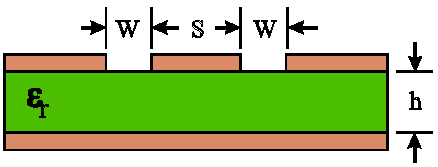
\includegraphics[width=0.6\textwidth]{figures/cpwg_drawing.pdf}
    \caption{Reproduced from \cite{ChemandyCalc}}
    \label{fig:CPWcross}
\end{figure}

Physically speaking, the main parameters taken into account were the center conductor width and the gap to the ground of the waveguide such as what is shown in \cref{fig:CPWcross} which, as discussed in \cref{GeneralCPW}, are the main contributing factors to the resonator's $Z_0$; as well as the total length of the resonator and the distance between the resonators and the feedline, which would in turn be the main contributing factors to the resonance frequency and the $Q_e$ accordingly.

A first estimation of the parameters was done using the expressions \cref{impedance,permittivity} for the $\epsilon_{eff}$ which is directly related to the $f_r$ and the $Z_0$. At the same time, an initial set of reference parameters was taken from a study carried out by \cite{Biznarova2024}, which proved to be the layout with the highest $Q_i$ in the aforementioned review by \cite{Ghione1987}, in the particular case of 2D aluminum circuits. This initial set of parameters was of 20$\mu m$ and 10$\mu m$ for the center conductor width ($w$) and the gap to ground ($g$) respectively, and an aluminum thickness of 300nm. Due to the reference setup being of aluminum over silicon, the values for $w$ and $g$ were adapted for each of the substrates to be studied.

As it is shown \textcolor{red}{in the Theory chapter}, both the $\epsilon_{eff}$ and the $Z_0$ come mainly given by the geometry of the CPW and the $\epsilon_r$ of the substrate. Therefore, the parameters mentioned in the previous paragraph were adapted for the values of $\epsilon_r$ for diamond, 4H-SiC and 6H-SiC that were retrieved from references \cite{Griesmayer, Li2024, Patrick1970} respectively, which was 5.7 for diamond; and in the case of the two kinds of SiC, due to being anisotropic materials, 9.77 for the ordinary axis and 10.2 for the extraordinary axis for 4H-SiC; and for 6H-SiC 9.66 for the ordinary axis and 10.3 for the extraordinary axis; in the cases of SiC, the xy-plane of the substrate was taken as parallel to the ordinary axis for the purpose of calculations. The adjusted values of both $w$ and $g$ were finally 20$\mu m$ and 10$\mu m$ respectively for both SiC orientations, and 20$\mu m$ and 4$\mu m$ respectively for diamond.

\subsection{Simulation iterations} \label{SimIterations}

After estimating these initial parameters, a series of numerical simulations were carried out using the method of moments software Sonnet Software. These simulations served as a way to tweak the estimation of the $f_r$ of each resonator; as well as a way to study the behavior of the relationship between $Q_e$ and the coupling distance ($d_c$). In order to carry out these simulations a reduced layout containing a single resonator and the feedline measuring 1920 $\times$ 2907.5 mm was used. This layout was divided using a rectangular mesh with a cell size of $2\times2 \mu m$; taking into account that the smallest distance in the SiC designs was 10$\mu m$; and in the case of the diamond design 4$\mu m$. It is of interest that even though a conformal mesh would have provided more accurate results, a rectangular mesh was used due to great increases of simulation time with the former. In order to carry out the desired assessment of the chips including a general study of the S21 response, the $Z_0$ and the $\epsilon_{eff}$, adaptive frequency sweeps were implemented in an interval close to the predicted $f_r$.

This process was done in an iterative manner; where, for each resonator of each substrate, firstly a coarse frequency sweep of 300 points was done in order to adjust the length of the resonator taking into account the $\epsilon_{eff}$ calculated by Sonnet and get closer to the desired $f_r$. Then, with the updated layout, a new coarse simulation was done in a 200MHz interval around an educated estimation of the $f_r$ in order to get a first indication of the power dip in the signal. Then, finer simulations of 600 and 800 points were done in progressively smaller intervals around the $f_r$ until the dip stopped growing vertically, which meant that the signal had been finely resolved closely around the $f_r$. Finally, the resolved signal was analyzed using the method developed by \cite{Lopez-Nunez2025}, which was useful to have a proper estimation of $Q_e$.

Through this process, the final parameters for the resonators were achieved. They can be found in \cref{tab:FinalParameters}

\subsection{Simulation results} \label{SimuResultsSection}

After the simulations were carried out, the overall behavior of the resonator described in \cref{GeneralCPW} was studied. This comprehensive study included the general electromagnetic behavior of the layout, such as voltage and current density along the CPW, and the resulting values of $\epsilon_{eff}$, and $Z_0$, which were consequently compared to those calculated from \cite{Wadell1991} used for the initial estimations mentioned in \cref{LayoutDesign}. Furthermore, it included an in-depth analysis of the $S_{21}$ spectrum following Lopez-Nuñez et al.'s method \cite{Lopez-Nunez2025} from which an estimation of $f_r$ and $Q_c$ was gotten. The numerical results of the simulations can be seen in \cref{tab:SimResults4H,tab:SimResults6H,tab:SimResultsdiamond}.

\begin{table}[ht]
    \centering
    \caption{Table with results from simulations and $S_{21}$ analysis for resonators with 4H-SiC substrate}
    \label{tab:SimResults4H}
    \begin{tabular}{@{}ccccccc@{}}
    \toprule\toprule
    Resonator & $f_{r, theory}$ & $f_{r, simulation}$ & $\epsilon_{theory}$ & $\epsilon_{simulation}$ & $Q_{c, theory}$ & $Q_{c, simulation}$ \\
    \midrule
    1         &                 &                     &                     &                         &                 &                     \\
    2         &                 &                     &                     &                         &                 &                     \\
    3         &                 &                     &                     &                         &                 &                     \\
    4         &                 &                     &                     &                         &                 &                     \\
    \bottomrule\bottomrule
    \end{tabular}
\end{table}

\begin{table}[ht]
    \centering
    \caption{Table with results from simulations and $S_{21}$ analysis for resonators with 6H-SiC substrate}
    \label{tab:SimResults6H}
    \begin{tabular}{@{}ccccccc@{}}
    \toprule\toprule
    Resonator & $f_{r, theory}$ & $f_{r, simulation}$ & $\epsilon_{theory}$ & $\epsilon_{simulation}$ & $Q_{c, theory}$ & $Q_{c, simulation}$ \\
    \midrule
    1         &                 &                     &                     &                         &                 &                     \\
    2         &                 &                     &                     &                         &                 &                     \\
    3         &                 &                     &                     &                         &                 &                     \\
    4         &                 &                     &                     &                         &                 &                     \\
    \bottomrule\bottomrule
    \end{tabular}
\end{table}

\begin{table}[ht]
    \centering
    \caption{Table with results from simulations and $S_{21}$ analysis for resonators with diamond substrate}
    \label{tab:SimResultsdiamond}
    \begin{tabular}{@{}ccccccc@{}}
    \toprule\toprule
    Resonator & $f_{r, theory}$ & $f_{r, simulation}$ & $\epsilon_{theory}$ & $\epsilon_{simulation}$ & $Q_{c, theory}$ & $Q_{c, simulation}$ \\
    \midrule
    1         &                 &                     &                     &                         &                 &                     \\
    2         &                 &                     &                     &                         &                 &                     \\
    3         &                 &                     &                     &                         &                 &                     \\
    4         &                 &                     &                     &                         &                 &                     \\
    \bottomrule\bottomrule
    \end{tabular}
\end{table}

It is interesting to point out how the simulated values of $\epsilon_{eff}$ and $Z_0$ systematically land higher than the ones calculated through the expressions derived from \cite{RaineeN2001}. This can be explained by the fact that in Wadell's equations\cite{Wadell1991}, there are several approximations that take place. Firstly, the ground surface around the resonator is approximated to be infinite; and, secondly, the metal is approximated to have a null thickness. 

These differences between the expected results and the ones retrieved from the simulations were studied. In the case of the metal thickness approximation, in \cite{RaineeN2001}, it is shown how, if the thickness of the metal is considered, as the metal thickness goes up, the predicted value of $\epsilon_{eff}$ becomes higher than the one expected from the initial conformal mapping expressions, and the value of $Z_0$ becomes lower than the one expected. On the other hand, for the ground surface size approximation, it was found that, according to \cite{Ghione1987}, as the ground surface around the conductor line is accounted for as finite, the value of $Z_0$ goes up the smaller the ground surface size; this approximation did not seem to have a noticeable effect on the value of $\epsilon_{eff}$. This last approximation was tested through a test run using a layout with a bigger ground size, closer to the real size of the chips. The results adjusted to the value of $Z_0$ decreasing with the larger ground. In the same way, test simulations were run that proved the value of $\epsilon_{eff}$ to increase as the thickness becomes bigger.

Being that the value of $Z_0$ was higher than the one predicted from the initial expressions it is thought that the effects of the 300nm thickness were negligible in comparison to the effects of the increase in ground size. This can be mainly explained by the fact that the size of the ground in the layouts used for the simulations was around a fifth of the real size in the x axis and a third of the real size in the y axis, and a thickness of 300nm results in a very small relation between the cross-section surface and the total length of the resonator.

\begin{figure}[h]
    \centering
    % \begin{subfigure}{0.32\textwidth}
    %     \includegraphics[width=\linewidth]{figures/diamond_in_res.png}
    %     \caption{Diamond, in resonance}
    %     \label{fig:diamond_in}
    % \end{subfigure}
    % \begin{subfigure}{0.32\textwidth}
    %     \includegraphics[width=\linewidth]{figures/4HSiC_in_res.png}
    %     \caption{4H-SiC, in resonance}
    %     \label{fig:4HSiC_in}
    % \end{subfigure}
    % \begin{subfigure}{0.32\textwidth}
    %     \includegraphics[width=\linewidth]{figures/6HSiC_in_res.png}
    %     \caption{6H-SiC, in resonance}
    %     \label{fig:6HSiC_in}
    % \end{subfigure}

    % \begin{subfigure}{0.32\textwidth}
    %     \includegraphics[width=\linewidth]{figures/diamond_out_res.png}
    %     \caption{Diamond, out of resonance}
    %     \label{fig:diamond_out}
    % \end{subfigure}
    % \begin{subfigure}{0.32\textwidth}
    %     \includegraphics[width=\linewidth]{figures/4HSiC_out_res.png}
    %     \caption{4H-SiC, out of resonance}
    %     \label{fig:4HSiC_out}
    % \end{subfigure}
    % \begin{subfigure}{0.32\textwidth}
    %     \includegraphics[width=\linewidth]{figures/6HSiC_out_res.png}
    %     \caption{6H-SiC, out of resonance}
    %     \label{fig:6HSiC_out}
    % \end{subfigure}

    \caption{Simulated surface current distribution in resonance (top row) and out of resonance (bottom row) for a representative resonator on each substrate. The distribution is dominated by the CPW geometry and is essentially substrate-independent. As discussed in \cref{GeneralCPW}, out of resonance, there is no energy transmission from the feedline to the resonator, and therefore no current density inside it. Also, in resonance, there is a maximum current density at the shorted end nearest to the feedline and a current density minimum at the open end, where there is a voltage maximum.}
    \label{fig:current_dist_all}
\end{figure}

Furthermore, the current density of the circuit can be seen in \cref{fig:diamond_in,fig:diamond_out,fig:6HSiC_in,fig:6HSiC_out,fig:4HSiC_in,fig:4HSiC_out}. These results become useful for confirmation of several points.

Furthermore, the current density of the circuit can be seen in \cref{fig:diamond_in,fig:diamond_out,fig:6HSiC_in,fig:6HSiC_out,fig:4HSiC_in,fig:4HSiC_out}. First, these results confirm that the resonator is only hosting the fundamental mode, as higher-order modes would be undesirable.

Second, they confirm the boundary conditions discussed in \cref{GeneralCPW}. At the shorted end, the impedance approaches zero, forcing the voltage to zero ($Z(0) \approx 0 \implies V(0) = 0$); which, by continuity of power flow, implies that the current there must instead be maximal. At the open end, the impedance diverges, forcing the current to zero ($Z(l) \to \infty \implies I(l) = 0$), while the voltage, and correspondingly the electric field, reaches its maximum. This is precisely the current maximum at the short and current minimum at the open end visible in each panel of \cref{fig:current_dist_all}.

Finally, this agreement extends to the three substrates, which was expected due to the analytical behavior only being explained through the geometry of the system and the only effects caused by the $\epsilon_r$ being on the $f_r$ and subsequently on the total length of the resonator rather than the shape of the standing wave.

\subsection{Fabrication of the resonators}

\subsubsection{Fabrication runs}

Once the final parameters were agreed to fit the general interests of this thesis they were sent out to the Max Planck Institute for Physics (MPP), which supplied the substrates to be studied. These substrates had the following specifications:

\begin{itemize}
    \item \textbf{Diamond substrate:} 
    
    Quantity: 2

    Dimensions: 4.5 mm $\times$ 4.5 mm $\times$ 0.5 mm

    Fabrication: Chemical vapor deposition (CVD)

    \item \textbf{4H-SiC substrate:}
    
    Quantity: 2

    Dimensions: 10 mm $\times$ 10 mm $\times$ 0.35 mm

    Fabrication: Chemical vapor deposition (CVD)

    \item \textbf{6H-SiC substrate:}
    
    Quantity: 2

    Dimensions: 10 mm $\times$ 10 mm $\times$ 0.35 mm

    Fabrication: Chemical vapor deposition (CVD)

\end{itemize}

The fabrication process carried out at MPP was divided in two runs. Firstly, an attempt using wet etching over a positive resist was made. This attempt turned out to be inconsistent due to the viscosity of the etchant being too high for the 10 $\upmu$m and 4 $\upmu$m crevices and therefore unreliable. The results were therefore discarded. 

Secondly, a lift-off run was tried. This second run resulted in a successful fabrication attempt for the SiC substrates, where the shape of the resonators was properly resolved, and the resist could be properly developed out of the sample's surface. For the diamond substrates both runs resulted in faulty circuits.

The process of the first run was carried out with the following steps:

\begin{enumerate}
    \item The substrates were cleaned using an HF bath, which is crucial to ensure a clean interface with the Al that will not tamper with the $Q_i$ results.
    \item An even 300 nm thick Al film was deposited on the samples using electron-beam evaporation under high vacuum conditions (UHV e-beam evaporation).
    \item Spin-coating using micro resist technology's positive resist ma-P 1215 was done on each substrate.
    \item The resist was exposed using a Heidelberg Instruments' $\upmu$MLA laser writer following the layout shown in \cref{fig:PositiveResist}. This way the area where the Al coating was desired was protected by the resist.
    \item The resist was developed using micro resist technology's ma-D 532/S.
    \item Wet etching was carried out using phosphoric-acetic-nitric acid mixture (PAN etching).
    \item The resist was stripped
\end{enumerate}

Furthermore, the process of the second run went as follows:

\begin{enumerate}
    \item The substrates were cleaned using an HF bath.
    \item Spin-coating using micro resist technology's negative resist ma-N 1440 was done on each substrate.
    \item The resist was exposed using the aforementioned $\upmu$MLA laser writer following the layout shown in \cref{fig:NegativeResist}. This way, the area of the substrate where the aluminum film was desired was left exposed, and the metal would not stick to the areas where the resist remained.
    \item The resist was developed using micro resist technology's ma-D 333/S.
    \item An even 300 nm Al film was deposited using the same UHV e-beam evaporation technique used in the first run.
    \item The remaining resist was lifted off along with the Al deposited on top of it.
\end{enumerate}

\subsubsection{Fabrication results}

Once the second fabrication run was finished, the four SiC chips which were checked with a microscope at MPP, and looked to be ready for measurements, were sent to IFAE's QCT workshop by mail. The chips were sent in standard \textcolor{red}{gel box}, wrapped in bubble wrap. Once they arrived they were revised using a microscope with \textcolor{red}{magnification} in order to have an idea of the chip's viability for measurement. In particular, the chips were checked for any short-circuit or discontinuities caused by a broken CPW line or by faulty fabrication; as well as debris or pieces of resist remaining due to an incomplete strip.

\textcolor{blue}{Afterward, a more in-depth visual study was carried out on a microscope with \textcolor{red}{magnification}. This was done in order to check for more precise information on the fabrication quality. This way aspects such as resolution, Al quality and presence of debris or remaining resist could be conclusively assessed.}

While looking at the chips with the first microscope, several defects were noticed. Especially, the feedline of the two 4H-SiC chips as well as one of the 6H-SiC chips, looked to be either completely broken at least at one point, or severely compromised by remaining resist. The remaining 6H-SiC chip was considered to be in proper conditions for measurement.

\textcolor{blue}{Moreover, the images taken of the chips can be seen in \cref{fig:Microscope}. In these images the overall resolution of the lift-off process can be assessed. Also, several images of the defects seen in the first assessment can be observed clearly.}

All in all, as it was expected from a first prototype, only one of the four chips that were received were expected to be functional.

\subsection{Measurements planning and setup}

Once the chips were obtained and available for measurement, it was of great importance to adjust the measurement setup to the experiment at hand. For this, the key aspects of the experiment had to be taken into account. These included the fact that the experiment was thought for superconducting Al, which meant its critical temperature ($T_c$) had to be taken into account; and the kind of measurements to be carried out, which were frequency and power sweeps seeking an in-depth study of the $S_{21}$ spectrum of the resonators in order to then extract the internal quality factor.

\begin{figure}[h]
    \centering
    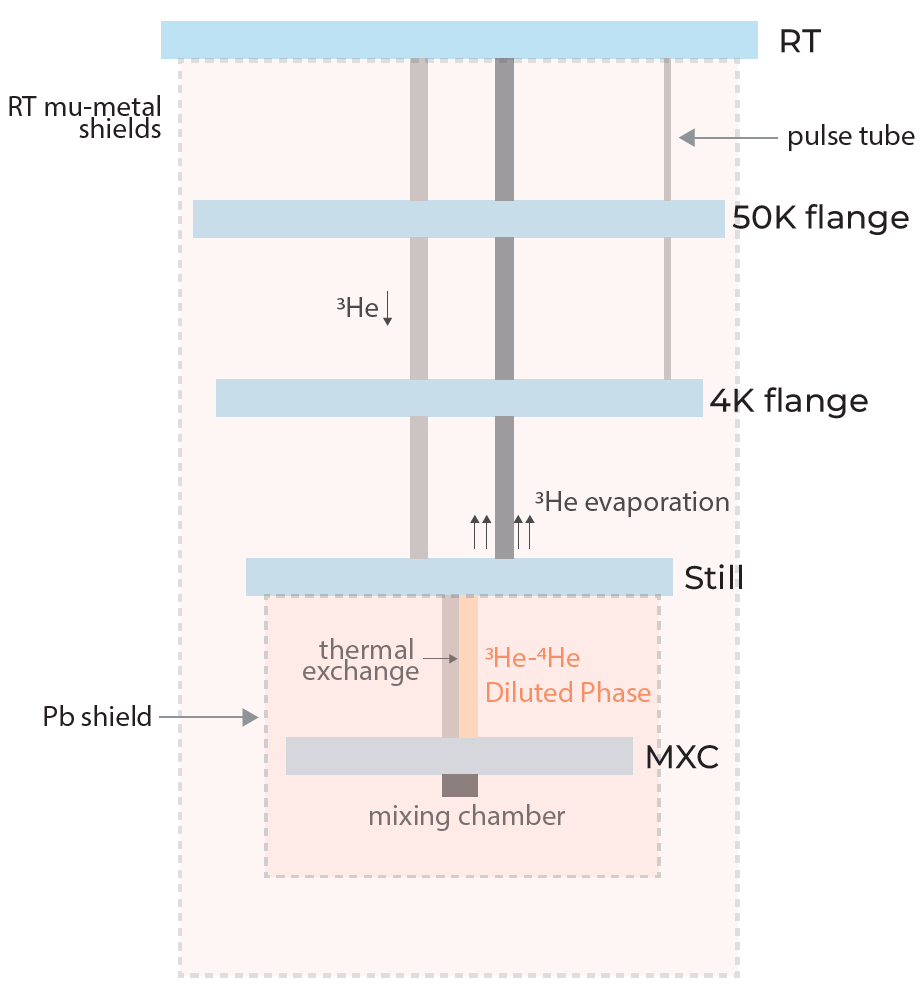
\includegraphics[width=0.4\textwidth]{figures/Fridge_cryo.png}
    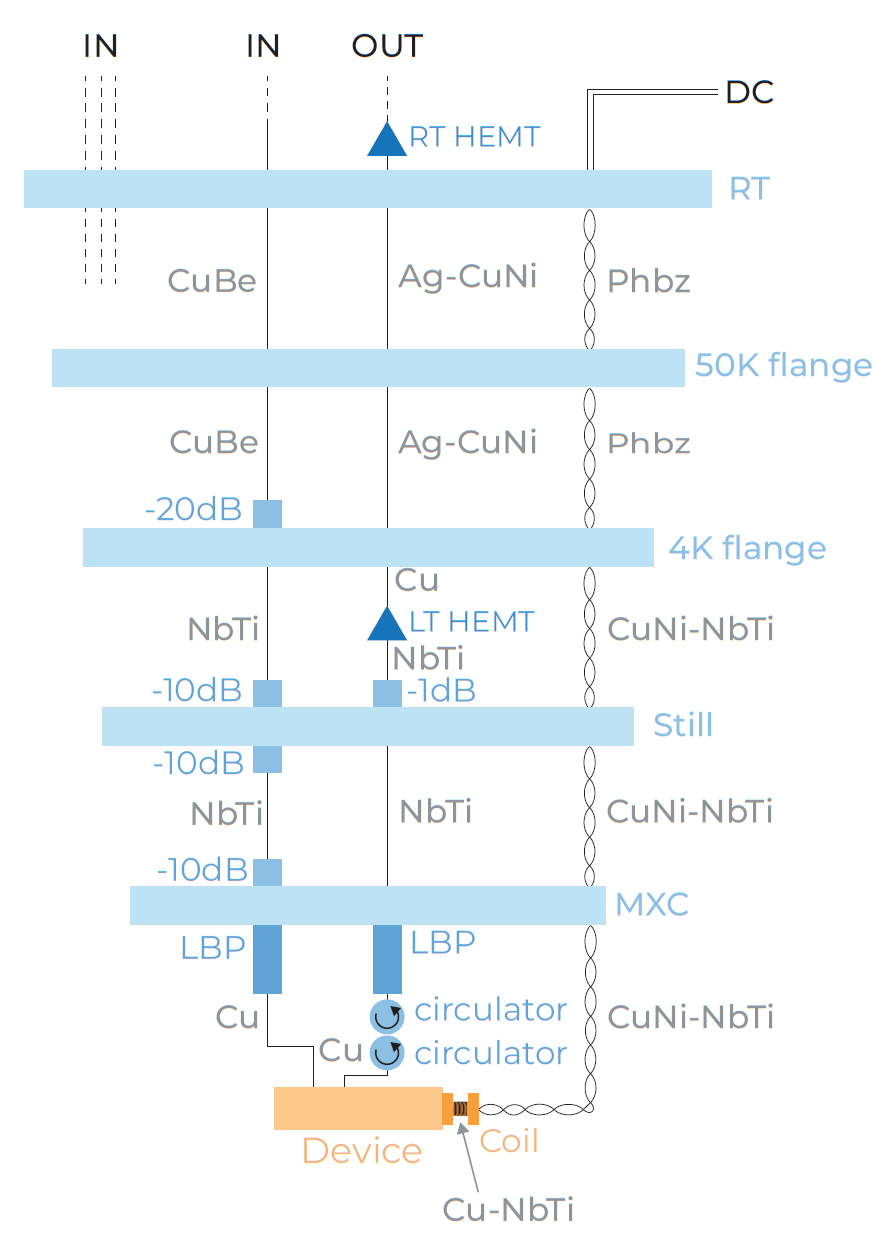
\includegraphics[width=0.4\textwidth]{figures/Fridge_circuit.png}
    \caption{Reproduced from \cite{LopezNunez2024}. Cryogenics schematics of Bluefors fridge, analogous to Leiden fridge setup. Circuitry schematics of Bluefors fridge, analogous to Leiden fridge setup.}
    \label{fig:Fridge}
\end{figure}

This experiment was planned to be carried out in a Leiden Cryogenics fridge using a setup like the one shown in \ref{fig:Fridge}. It is of interest that the stage where the chip is set to be measured will be at $\sim 20$K. Furthermore, the use of a Pb magnetic shield was thought to avoid losses due to external magnetic fields or external radiation.

Furthermore, in order to have proper control over the input signal and be able to measure the output properly a setup such as the one shown in \cref{fig:Fridge} was employed. In these schematics several attenuators can be observed between the input signal generator and the device; this is motivated by the fact that the power interval desired to work in is in the single photon regime. Also, low band pass filters can be seen right before and after the connection to the device; these filters serve as a way to prevent noise affecting the measurements.

Additionally, two \textcolor{red}{amplifiers} can be seen in the second stage of the fridge and right before the output acquisition. These amplifiers are crucial to the measurement of the device's response, as the power output has been diminished almost to zero by the attenuators on the input side of the circuit.

In order to study the same behaviors discussed in \cref{SimuResultsSection}, the measurement was planned to be as follows:

\begin{enumerate}
    \item A coarse frequency sweep around the respective $f_r$ of each resonator in order to find where the real dip was located.
    \item Once the dip was located, a finer sweep, closing in on the $f_r$ and with a higher intermediate frequency (IF) in order to better resolve the spectrum.
    \item Once a properly resolved $S_{21}$ spectrum is achieved, exporting the $\Re S_{21}$ and $\Im S_{21}$ spectrum.
    \item Using Lopez-Nuñez's method \cite{Lopez-Nunez2025}, extracting the desired data related to $Q_i$ as it is the interest of this thesis; as well as data related to $\epsilon_{eff}, Z_0$ and $Q_c$ in order to compare the results from the fabricated chips with those gotten from the Sonnet simulations.
\end{enumerate}

Additionally, in every step of this measurement plan, several iterations were planned to be carried out on each step, with increasingly less attenuation. This would then allow us to perform a sweep in power. This is of interest in order to later on be able to tell whether the energy losses where due to dielectric TLS.

This way, the resulting spectrum obtained from the measurements should look similar to those described in \cref{Qfactor,SimuResultsSection}. This means properly fitting the complex $S_{21}$ spectrum to the expression presented by Lopez-Nuñez, et al. \cite{Lopez-Nunez2025}.

The real $f_r$ are expected to fall slightly under the predicted values. Also, the experimental values of $Q_c$ are expected to vary significantly, especially at higher values, due to its high sensitivity to any variation in coupling distance.

Due to fabrication and cryostat scheduling constraints, the measurements explained were not carried out within the scope of this thesis. Further work to measure the chips discussed in this text is necessary; as well as future fabrication runs to make up for the unviable chips, including the diamond substrates and the 4H-SiC substrates. Discussions surrounding the development of a mask for each kind of substrate with intentions of fabricating larger wafers were taking place at the time of this work's end.

\section{Conclusions and outlook}



\newpage

\printbibliography[heading=bibintoc]

\end{document}


